\chapter{Signal Fits}\label{appendix_signal_fits}

\begin{figure}[htb]
	\begin{center}
		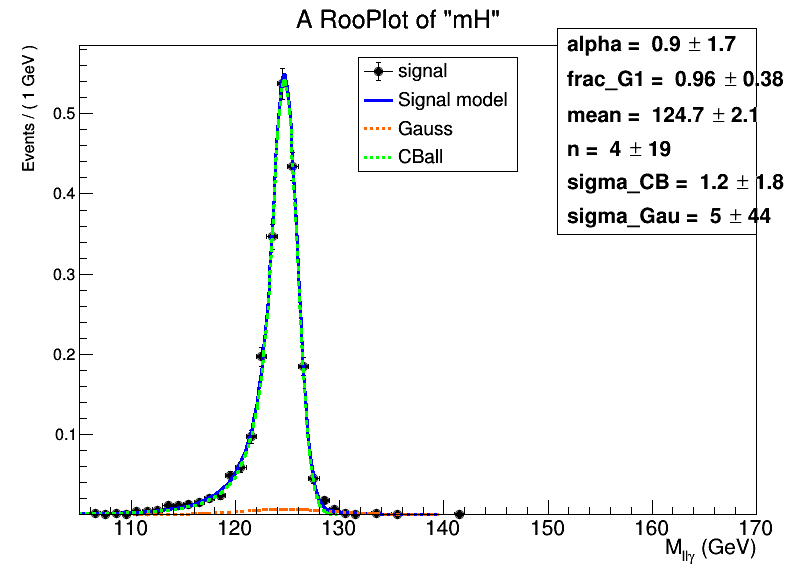
\includegraphics[width=0.25\textwidth]{fig/signal_fit/2016/sigfit_ele_ggF_1_125.png}
		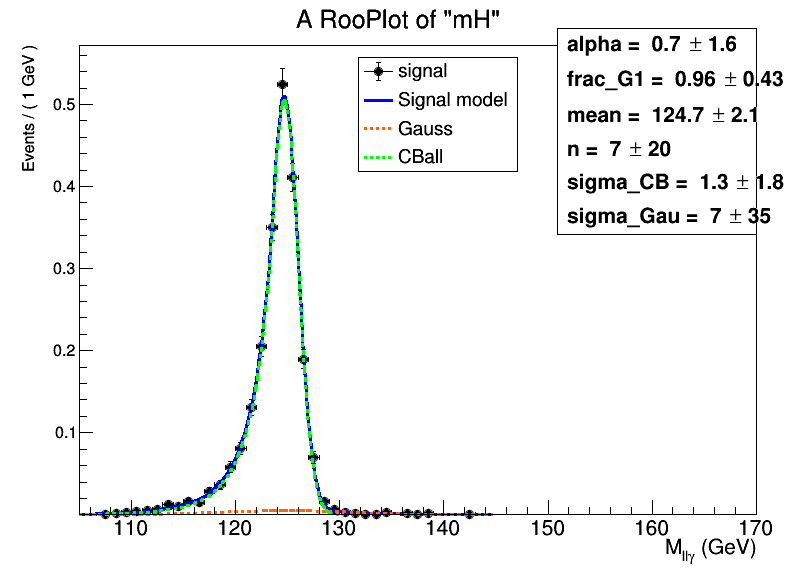
\includegraphics[width=0.25\textwidth]{fig/signal_fit/2016/sigfit_ele_ggF_2_125.png}\\
		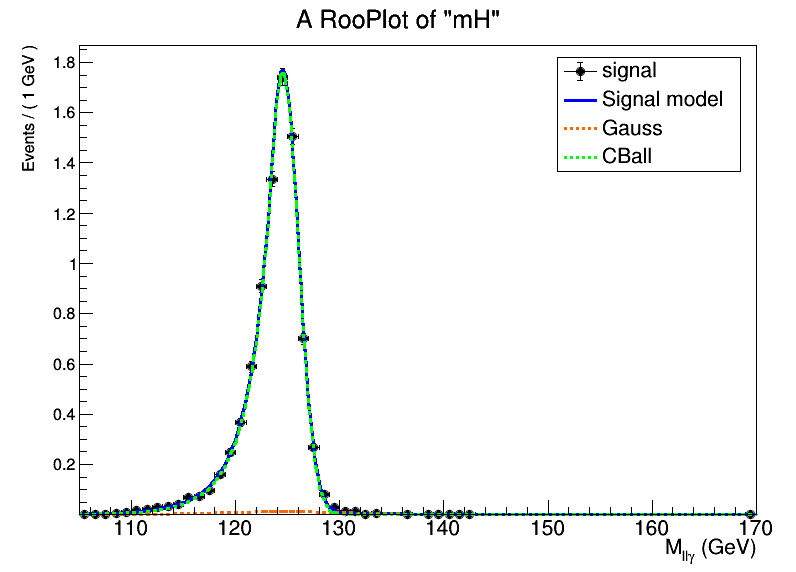
\includegraphics[width=0.25\textwidth]{fig/signal_fit/2016/sigfit_ele_ggF_3_125.png}
		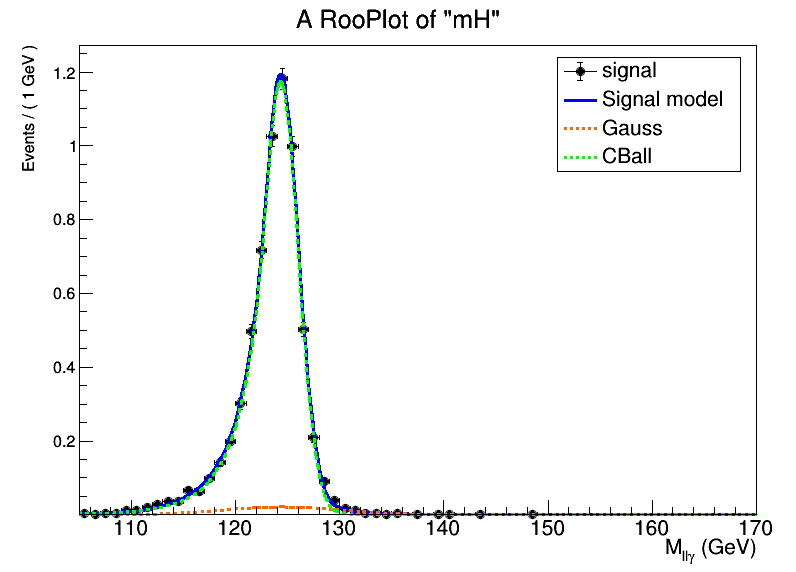
\includegraphics[width=0.25\textwidth]{fig/signal_fit/2016/sigfit_ele_ggF_4_125.png}\\
		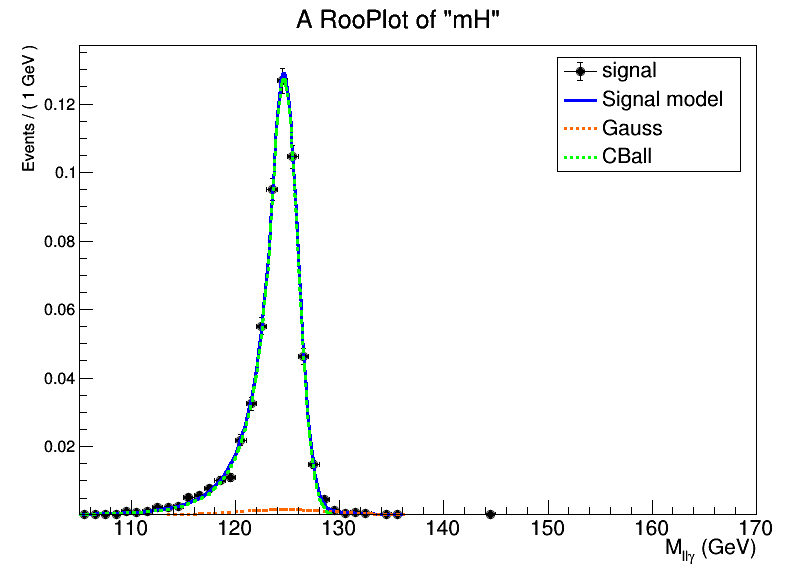
\includegraphics[width=0.25\textwidth]{fig/signal_fit/2016/sigfit_ele_VBF_501_125.png}
		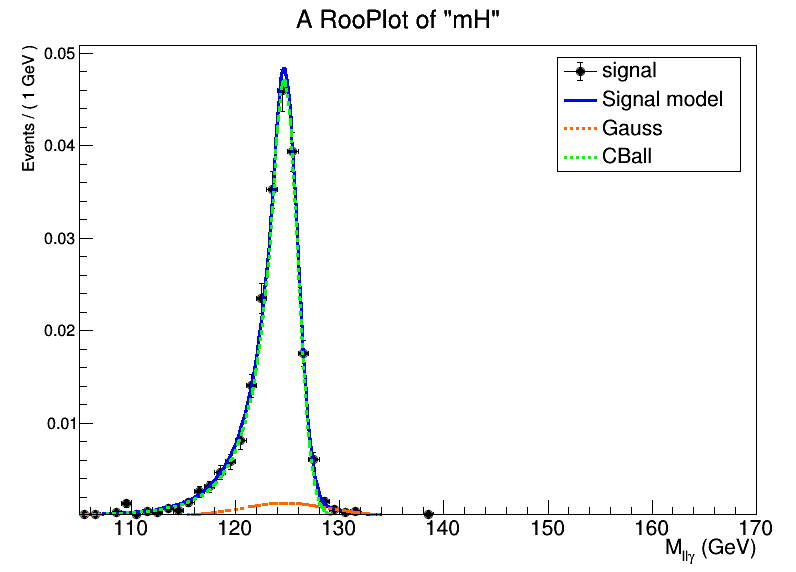
\includegraphics[width=0.25\textwidth]{fig/signal_fit/2016/sigfit_ele_VBF_502_125.png}\\
		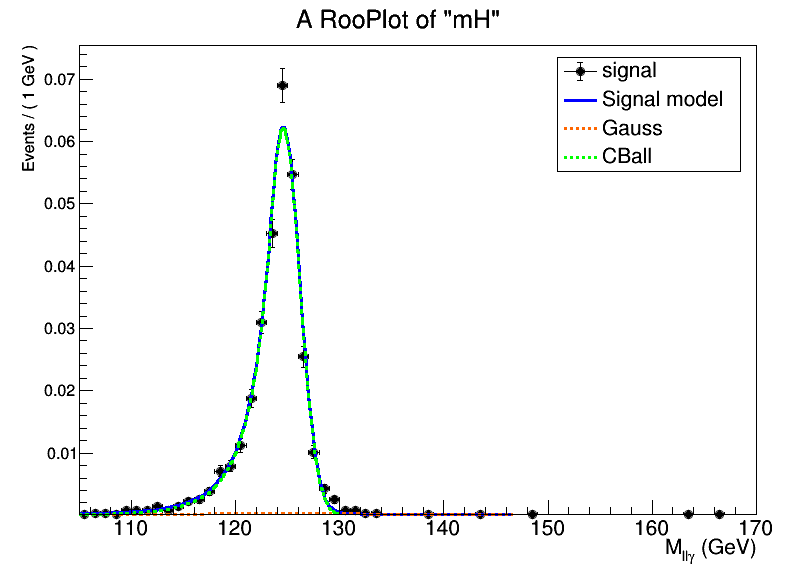
\includegraphics[width=0.25\textwidth]{fig/signal_fit/2016/sigfit_ele_VBF_503_125.png}\\
		\caption{Fits to simulated $m_{\ell^+\ell^-\gamma}$ signal distributions in the electron channel for
            		 $m_\PH=125\GeV$ for the 2016 data-taking period.
			 The top four plots correspond to the untagged categories, and the bottom three plots correspond to the dijet categories.}
		\label{fig:elesigfit_16}
	\end{center}
\end{figure}

\begin{figure}[htb]
	\begin{center}
		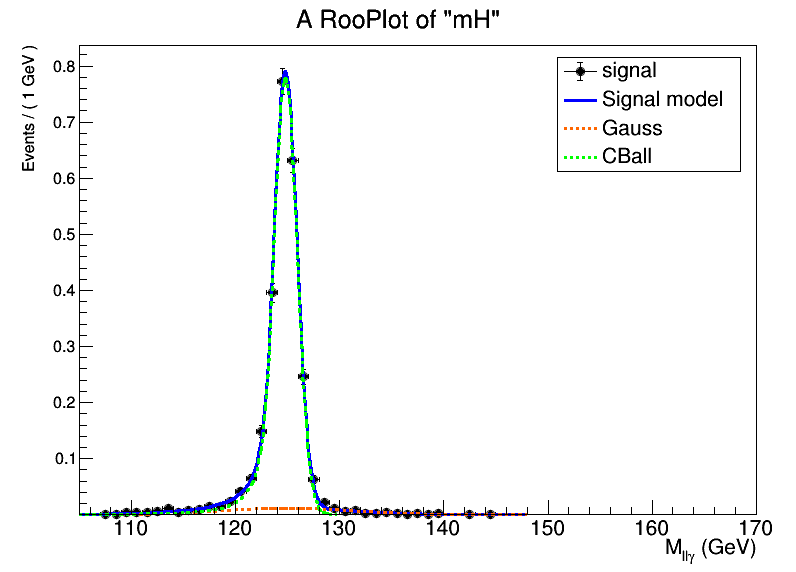
\includegraphics[width=0.40\textwidth]{fig/signal_fit/2016/sigfit_mu_ggF_1_125.png}
		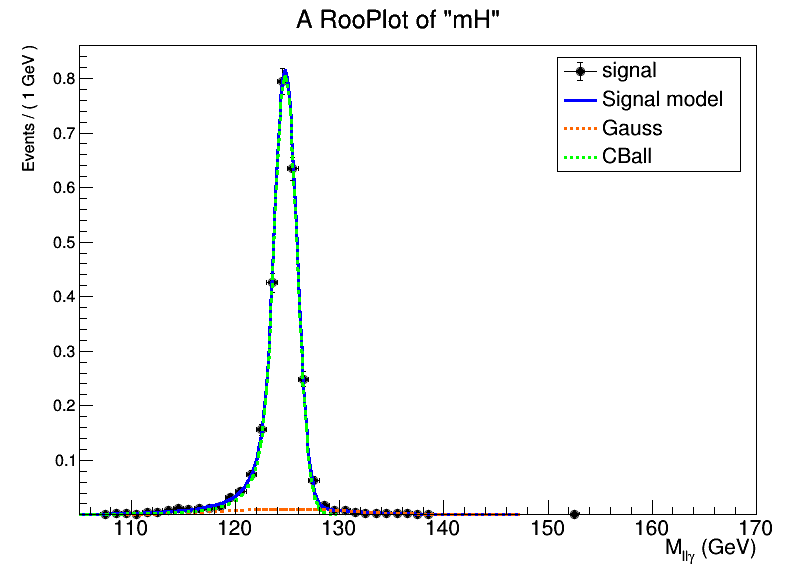
\includegraphics[width=0.40\textwidth]{fig/signal_fit/2016/sigfit_mu_ggF_2_125.png}\\
		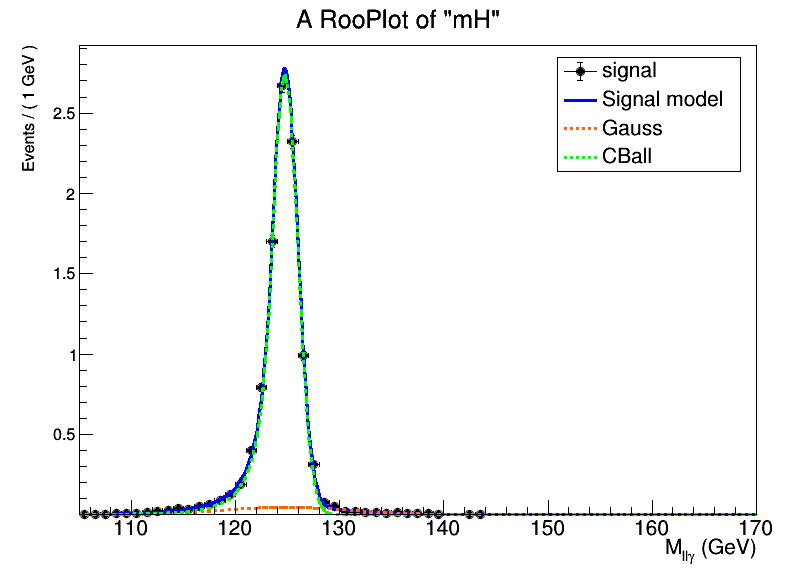
\includegraphics[width=0.40\textwidth]{fig/signal_fit/2016/sigfit_mu_ggF_3_125.png}
		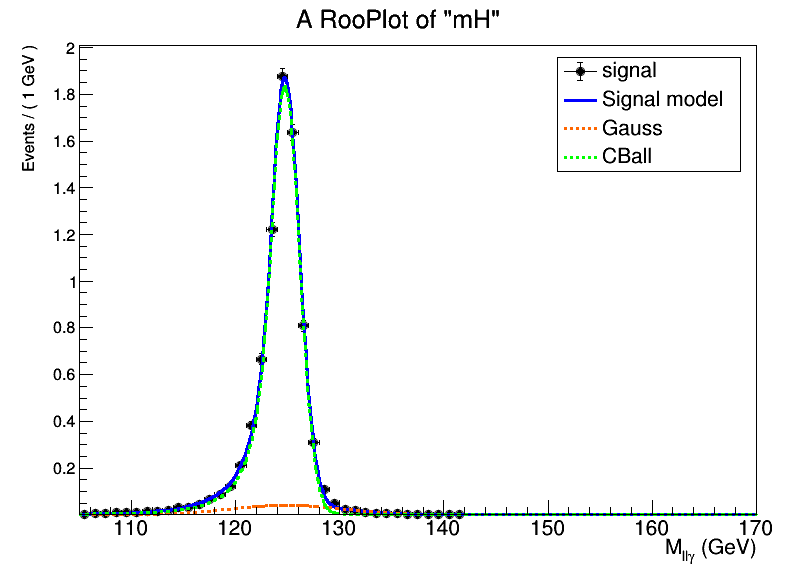
\includegraphics[width=0.40\textwidth]{fig/signal_fit/2016/sigfit_mu_ggF_4_125.png}\\
		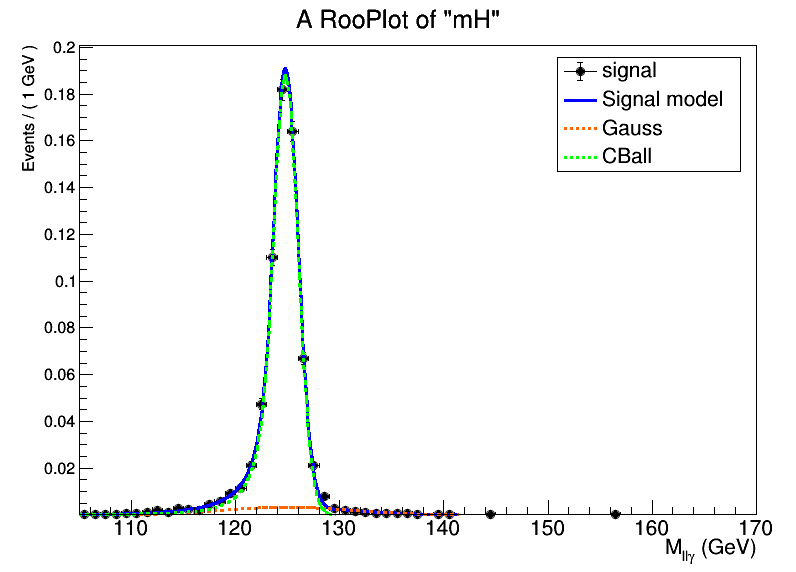
\includegraphics[width=0.40\textwidth]{fig/signal_fit/2016/sigfit_mu_VBF_501_125.png}
		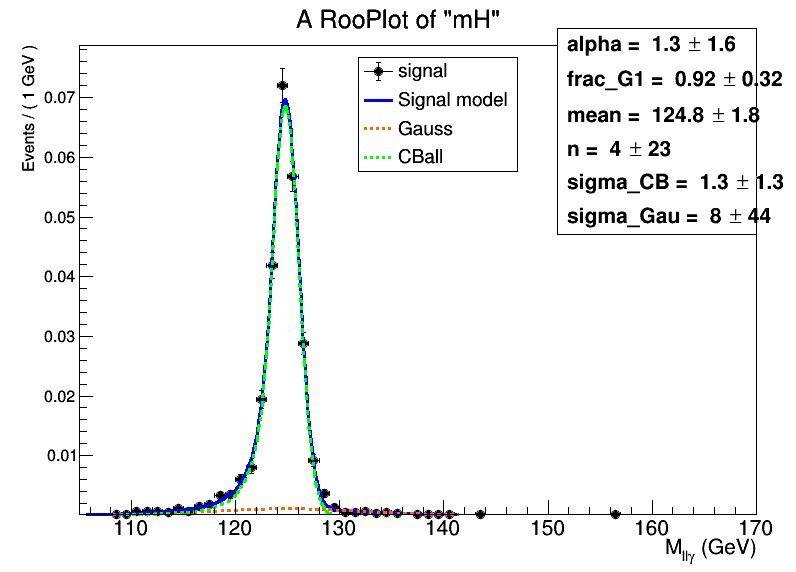
\includegraphics[width=0.40\textwidth]{fig/signal_fit/2016/sigfit_mu_VBF_502_125.png}\\
		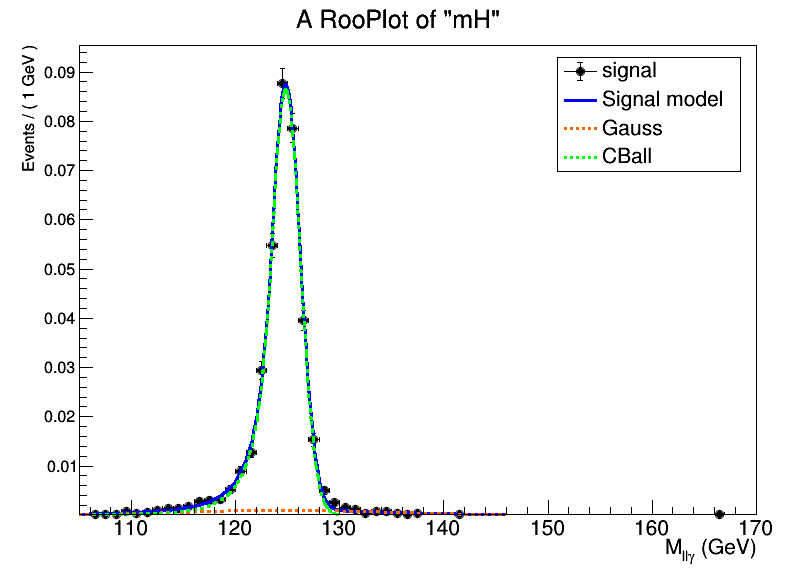
\includegraphics[width=0.40\textwidth]{fig/signal_fit/2016/sigfit_mu_VBF_503_125.png}\\
		\caption{Fits to simulated $m_{\ell^+\ell^-\gamma}$ signal distributions in the muon channel for
            		 $m_\PH=125\GeV$ for the 2016 data-taking period.
			 The top four plots correspond to the untagged categories, and the bottom three plots correspond to the dijet categories.}
		\label{fig:musigfit_16}
	\end{center}
\end{figure}

\begin{figure}[htb]
	\begin{center}
		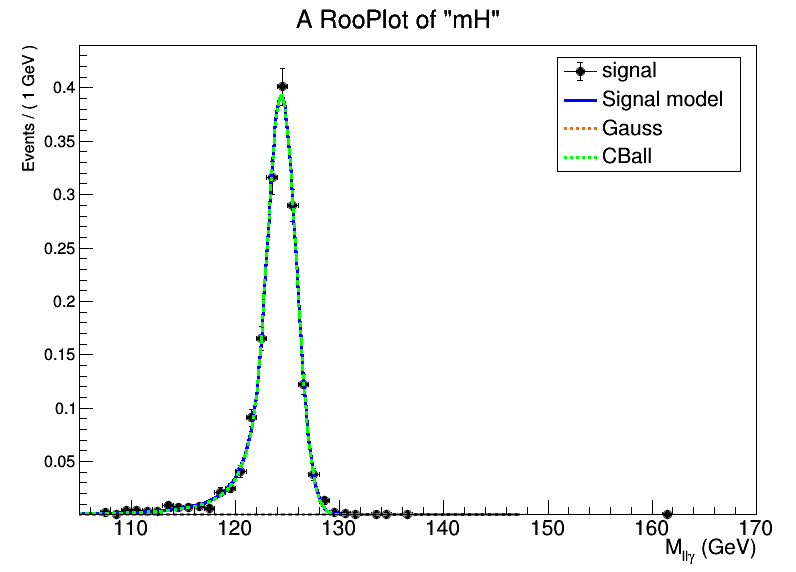
\includegraphics[width=0.40\textwidth]{fig/signal_fit/2017/sigfit_ele_ggF_1_125.png}
		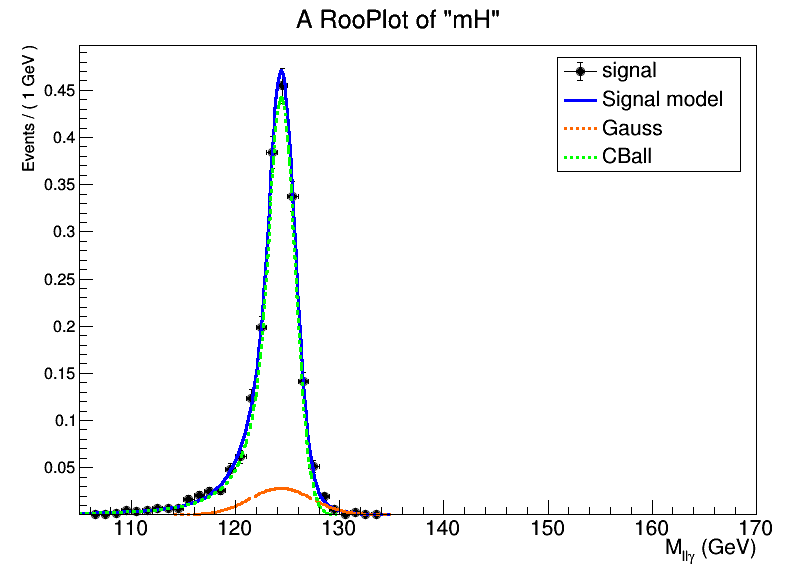
\includegraphics[width=0.40\textwidth]{fig/signal_fit/2017/sigfit_ele_ggF_2_125.png}\\
		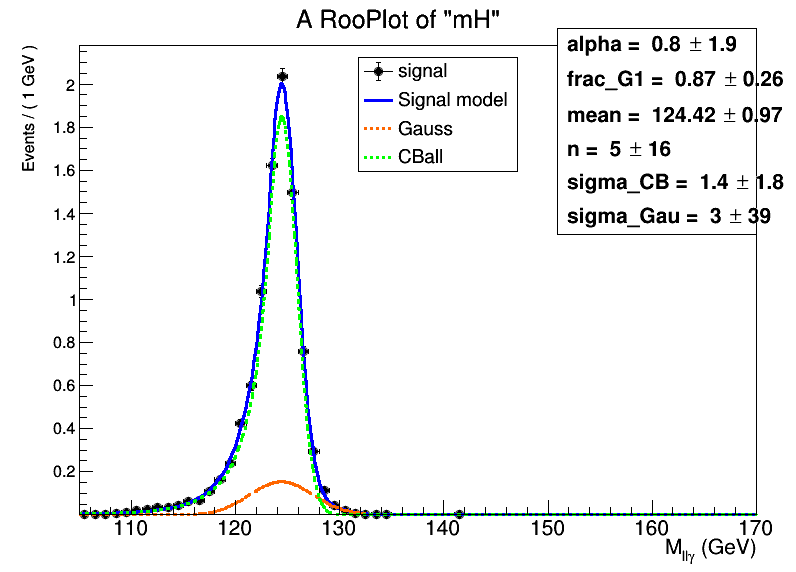
\includegraphics[width=0.40\textwidth]{fig/signal_fit/2017/sigfit_ele_ggF_3_125.png}
		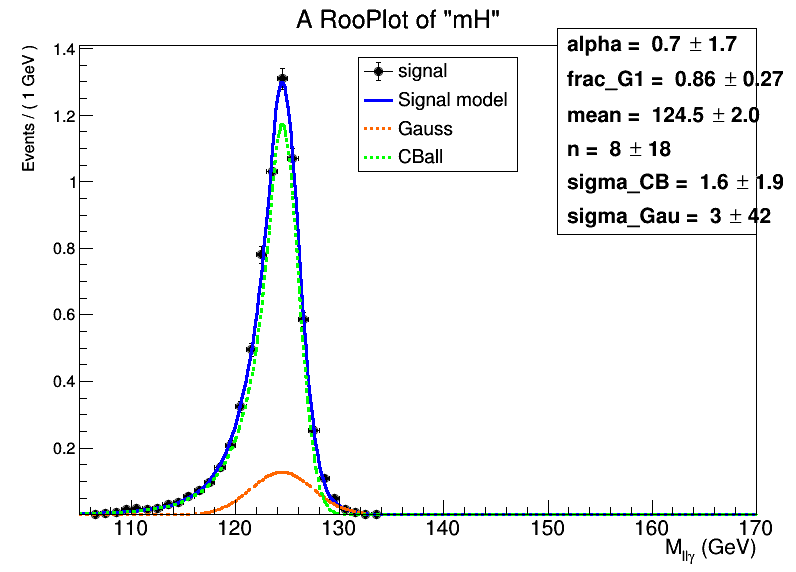
\includegraphics[width=0.40\textwidth]{fig/signal_fit/2017/sigfit_ele_ggF_4_125.png}\\
		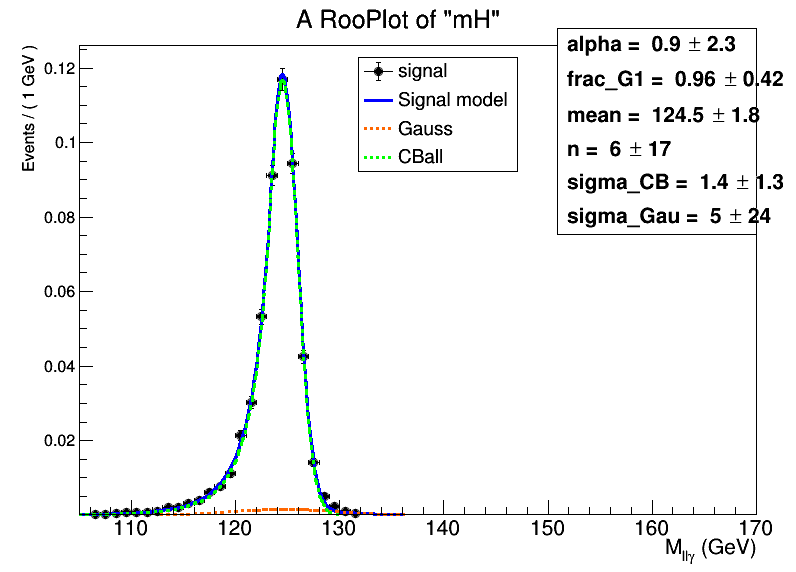
\includegraphics[width=0.40\textwidth]{fig/signal_fit/2017/sigfit_ele_VBF_501_125.png}
		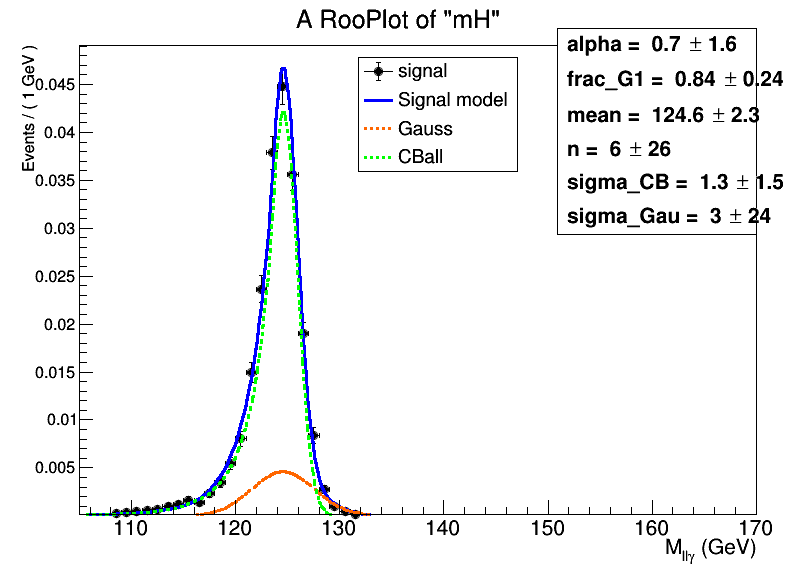
\includegraphics[width=0.40\textwidth]{fig/signal_fit/2017/sigfit_ele_VBF_502_125.png}\\
		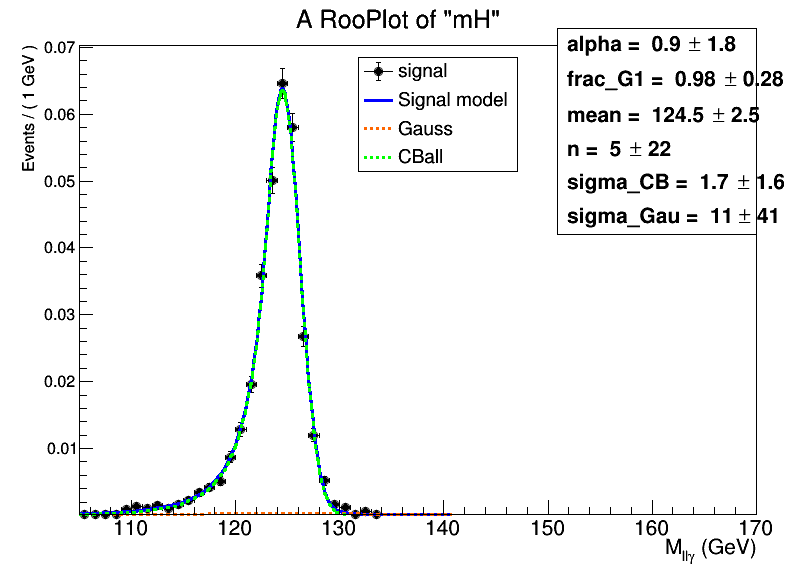
\includegraphics[width=0.40\textwidth]{fig/signal_fit/2017/sigfit_ele_VBF_503_125.png}\\
		\caption{Fits to simulated $m_{\ell^+\ell^-\gamma}$ signal distributions in the electron channel for
            		 $m_\PH=125\GeV$ for the 2017 data-taking period.
			 The top four plots correspond to the untagged categories, and the bottom three plots correspond to the dijet categories.}
		\label{fig:elesigfit_17}
	\end{center}
\end{figure}

\begin{figure}[htb]
	\begin{center}
		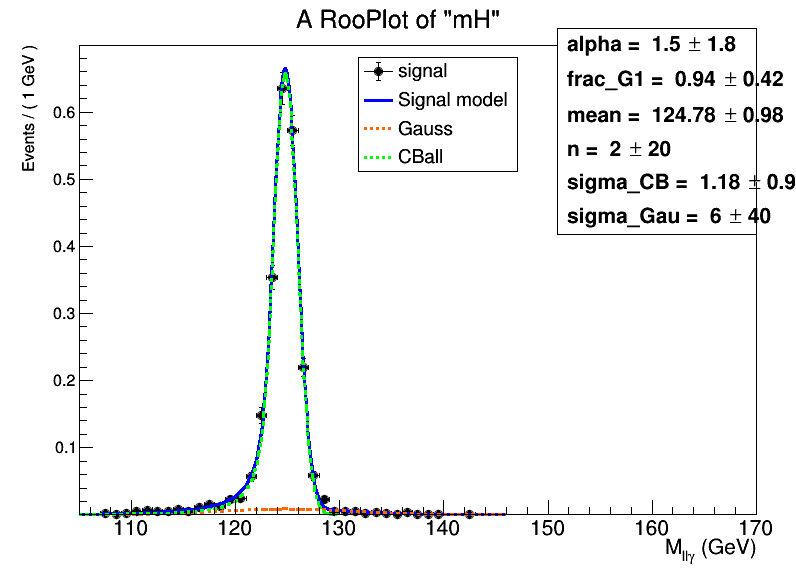
\includegraphics[width=0.40\textwidth]{fig/signal_fit/2017/sigfit_mu_ggF_1_125.png}
		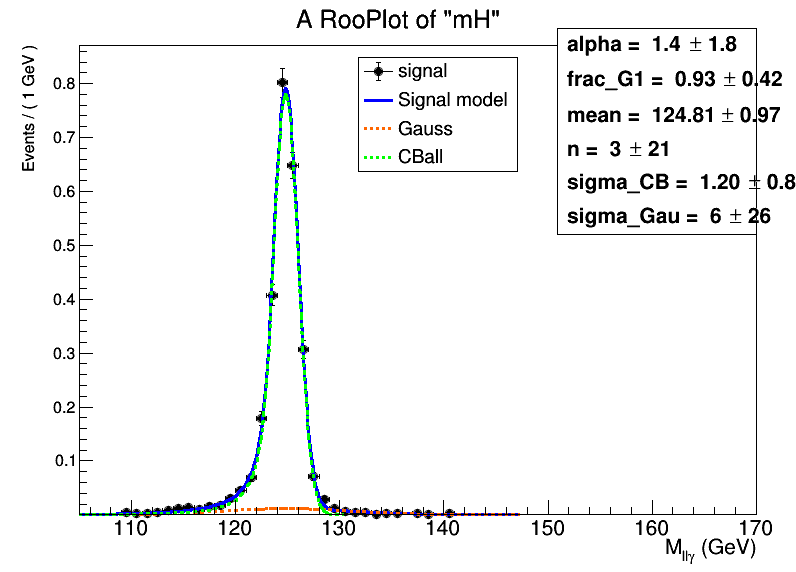
\includegraphics[width=0.40\textwidth]{fig/signal_fit/2017/sigfit_mu_ggF_2_125.png}\\
		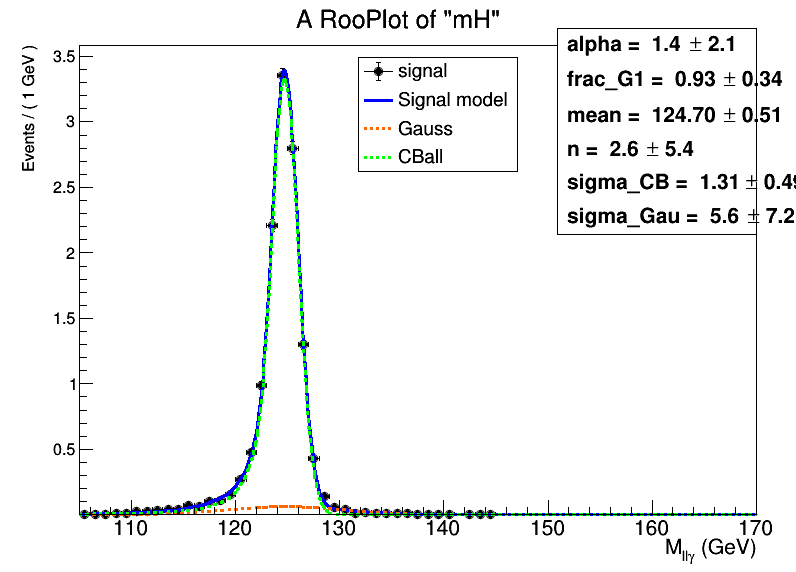
\includegraphics[width=0.40\textwidth]{fig/signal_fit/2017/sigfit_mu_ggF_3_125.png}
		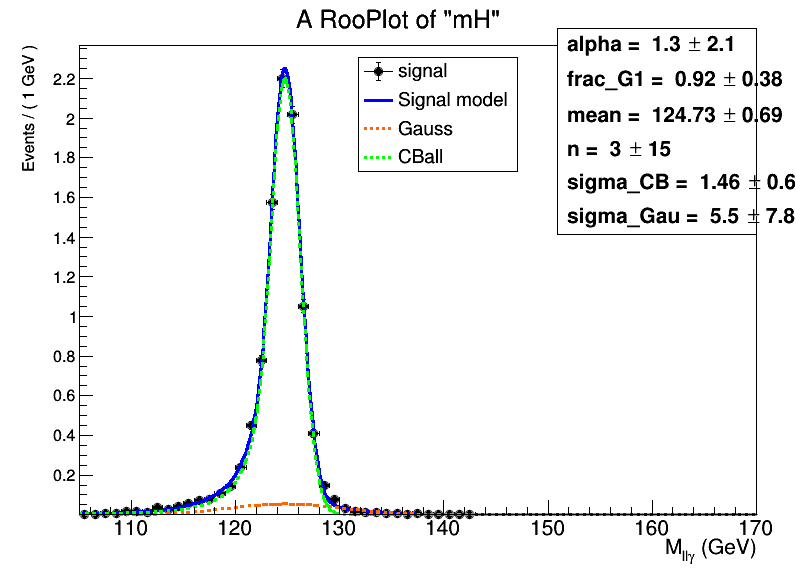
\includegraphics[width=0.40\textwidth]{fig/signal_fit/2017/sigfit_mu_ggF_4_125.png}\\
		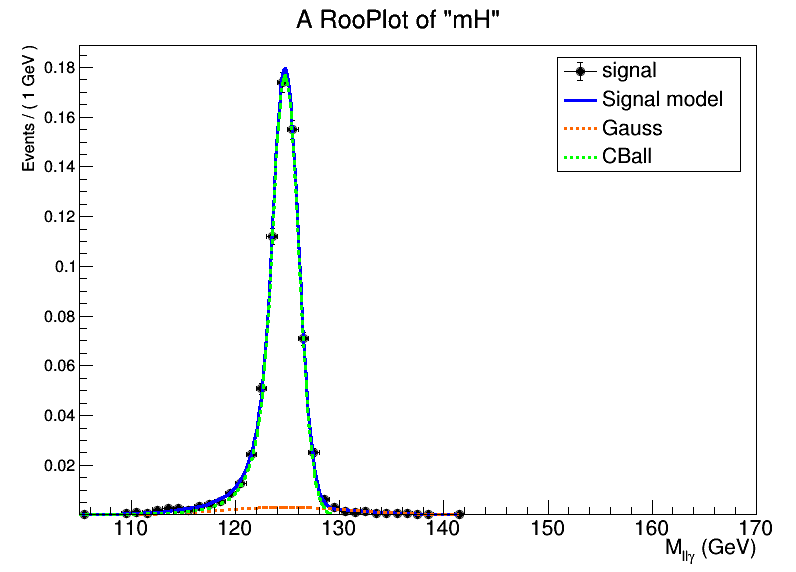
\includegraphics[width=0.40\textwidth]{fig/signal_fit/2017/sigfit_mu_VBF_501_125.png}
		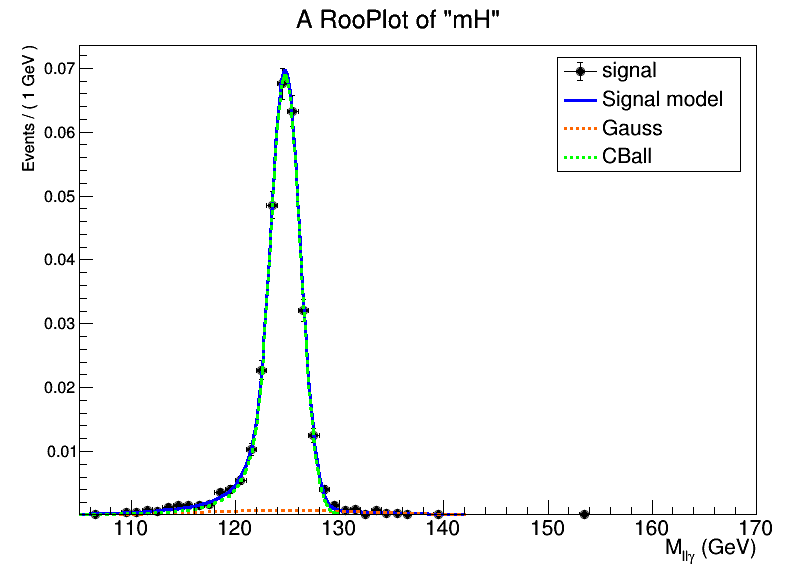
\includegraphics[width=0.40\textwidth]{fig/signal_fit/2017/sigfit_mu_VBF_502_125.png}\\
		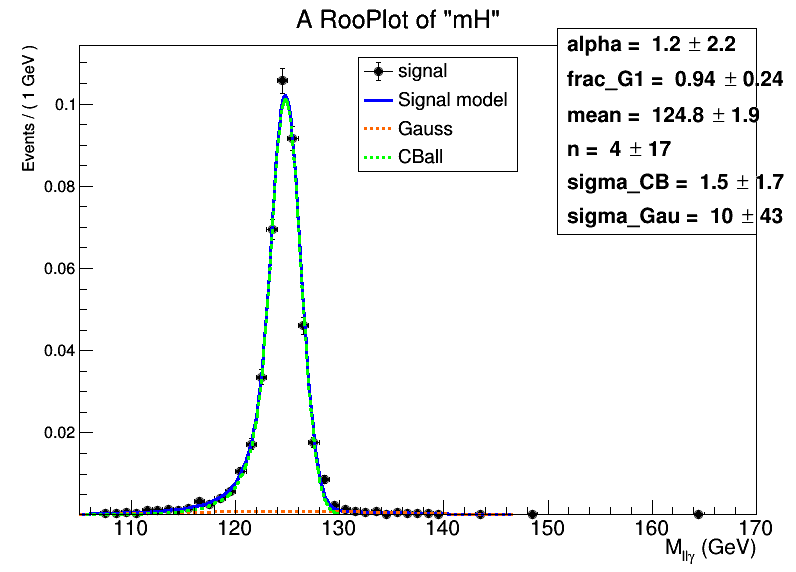
\includegraphics[width=0.40\textwidth]{fig/signal_fit/2017/sigfit_mu_VBF_503_125.png}\\
		\caption{Fits to simulated $m_{\ell^+\ell^-\gamma}$ signal distributions in the muon channel for
            		 $m_\PH=125\GeV$ for the 2017 data-taking period.
			 The top four plots correspond to the untagged categories, and the bottom three plots correspond to the dijet categories.}
		\label{fig:musigfit_17}
	\end{center}
\end{figure}

\begin{figure}[htb]
	\begin{center}
		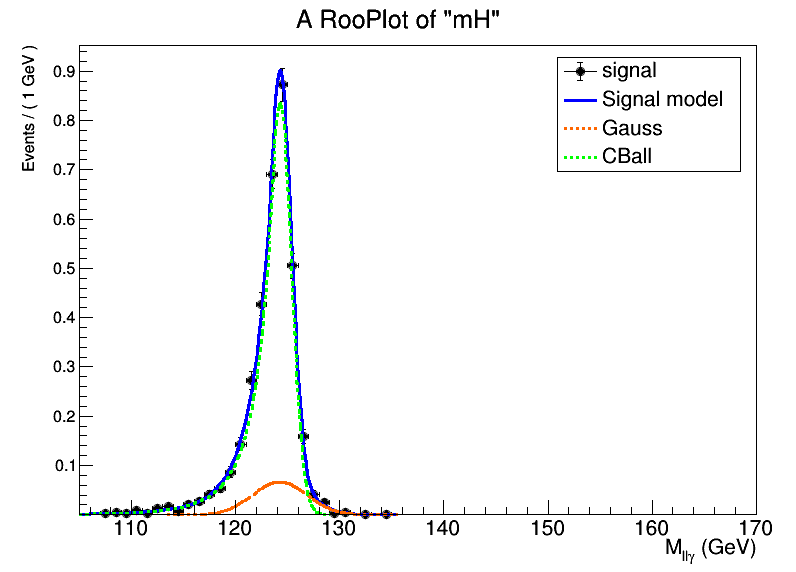
\includegraphics[width=0.40\textwidth]{fig/signal_fit/2018/sigfit_ele_ggF_1_125.png}
		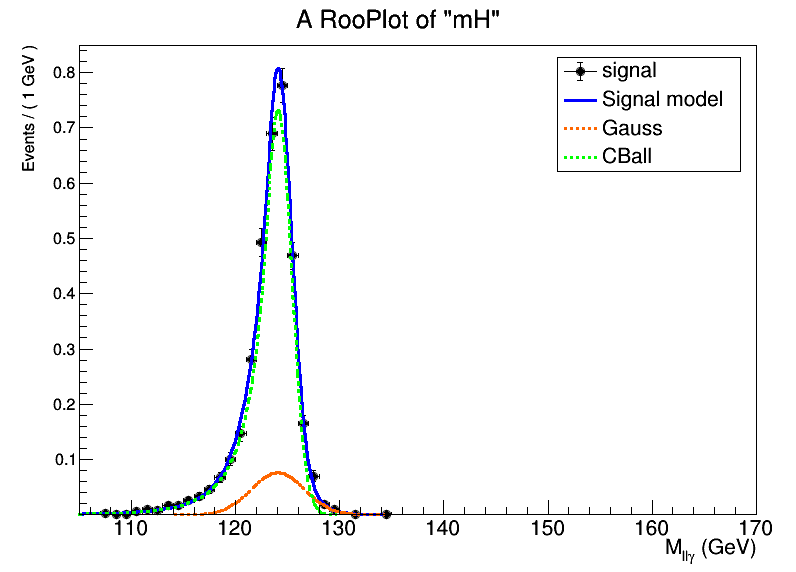
\includegraphics[width=0.40\textwidth]{fig/signal_fit/2018/sigfit_ele_ggF_2_125.png}\\
		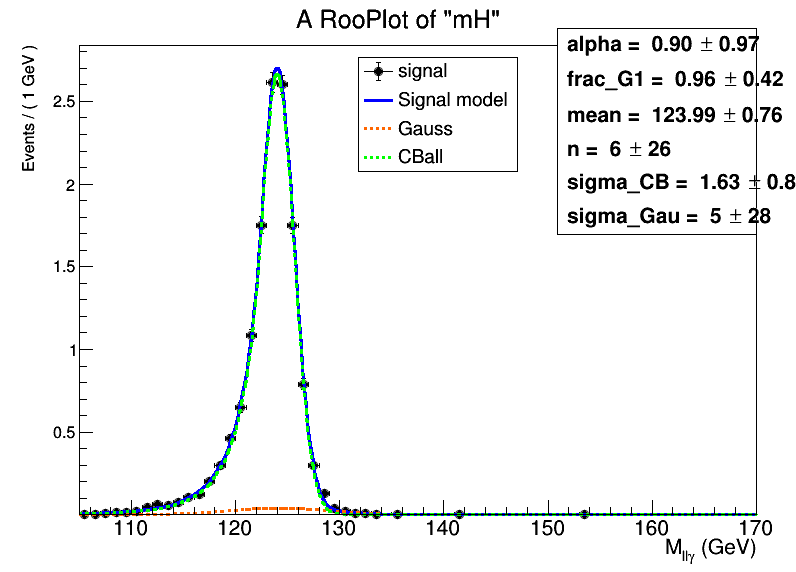
\includegraphics[width=0.40\textwidth]{fig/signal_fit/2018/sigfit_ele_ggF_3_125.png}
		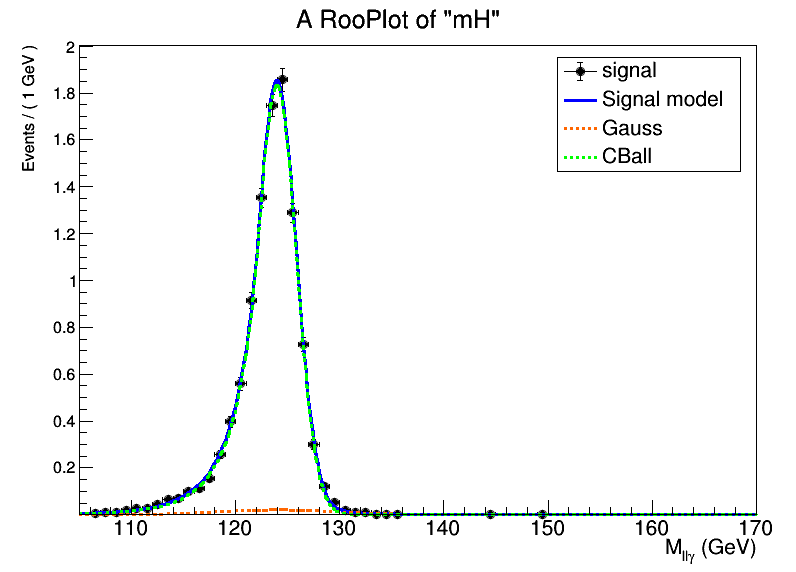
\includegraphics[width=0.40\textwidth]{fig/signal_fit/2018/sigfit_ele_ggF_4_125.png}\\
		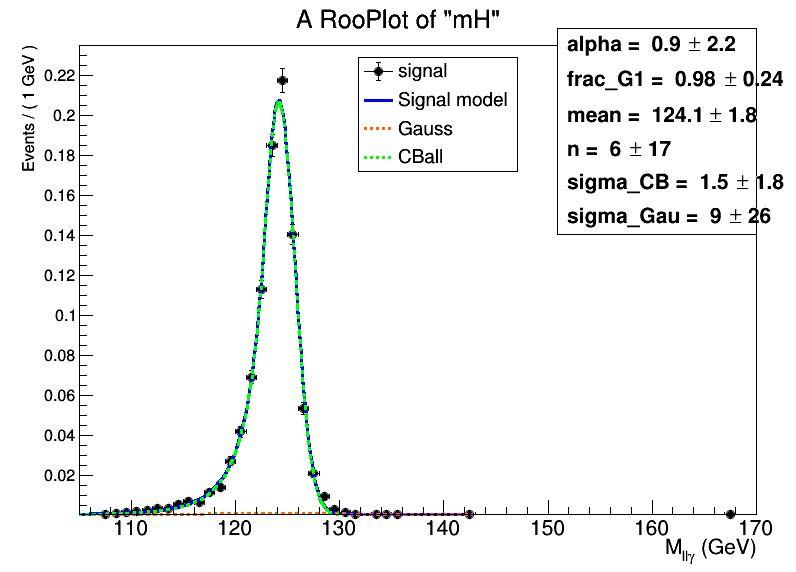
\includegraphics[width=0.40\textwidth]{fig/signal_fit/2018/sigfit_ele_VBF_501_125.png}
		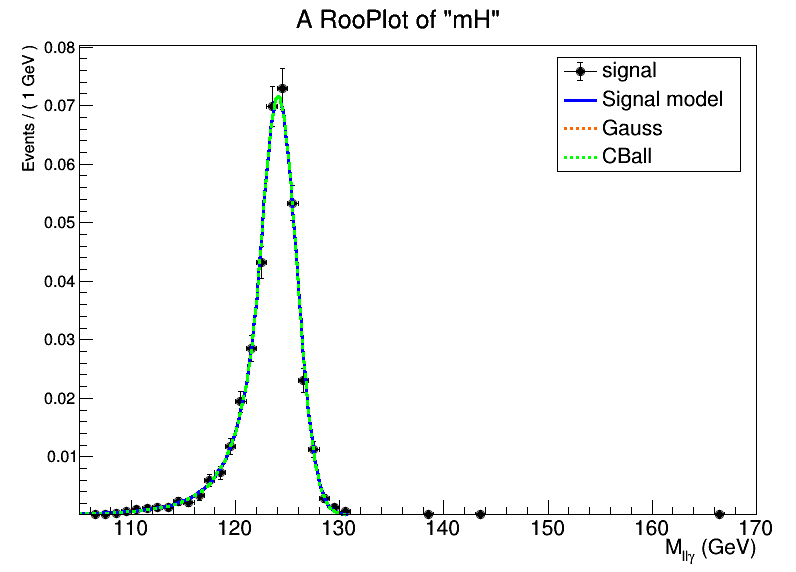
\includegraphics[width=0.40\textwidth]{fig/signal_fit/2018/sigfit_ele_VBF_502_125.png}\\
		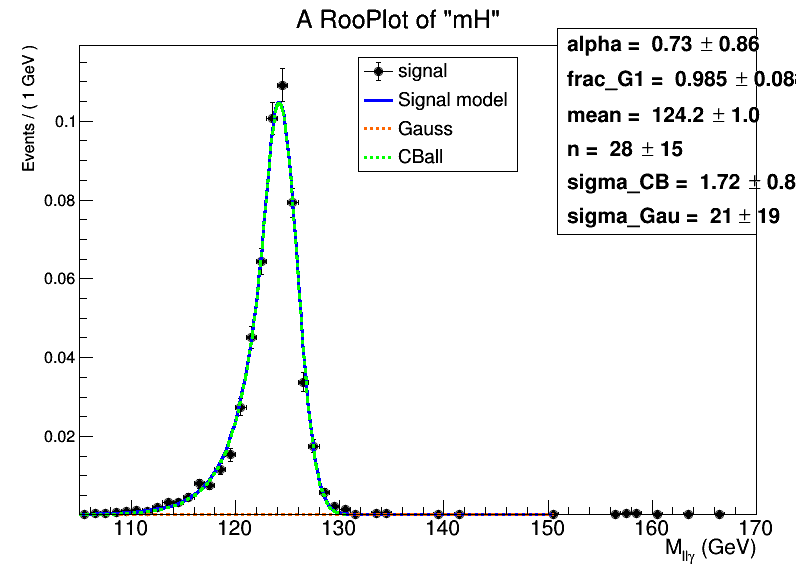
\includegraphics[width=0.40\textwidth]{fig/signal_fit/2018/sigfit_ele_VBF_503_125.png}\\
		\caption{Fits to simulated $m_{\ell^+\ell^-\gamma}$ signal distributions in the electron channel for
            		 $m_\PH=125\GeV$ for the 2018 data-taking period.
			 The top four plots correspond to the untagged categories, and the bottom three plots correspond to the dijet categories.}
		\label{fig:elesigfit_18}
	\end{center}
\end{figure}

\begin{figure}[htb]
	\begin{center}
		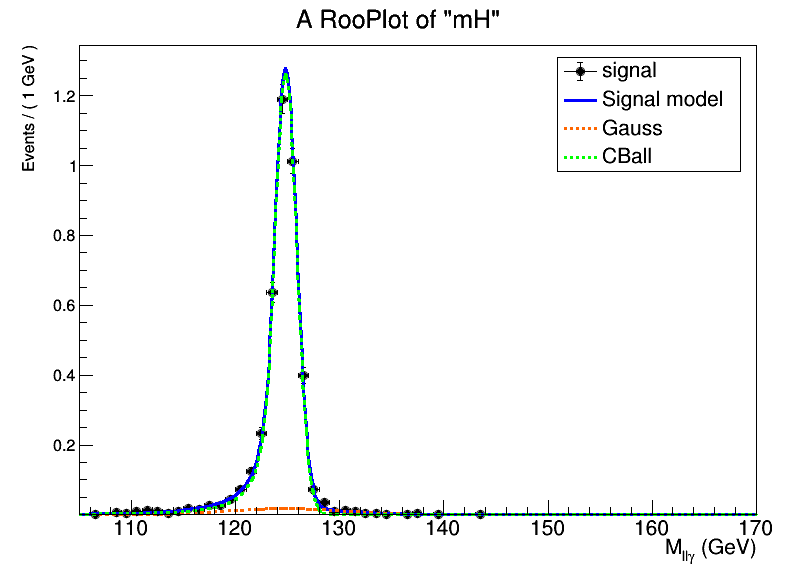
\includegraphics[width=0.40\textwidth]{fig/signal_fit/2018/sigfit_mu_ggF_1_125.png}
		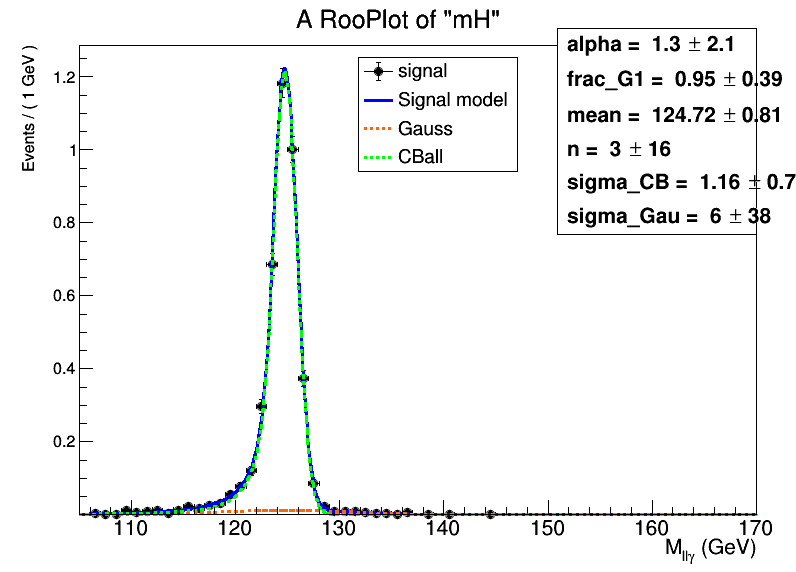
\includegraphics[width=0.40\textwidth]{fig/signal_fit/2018/sigfit_mu_ggF_2_125.png}\\
		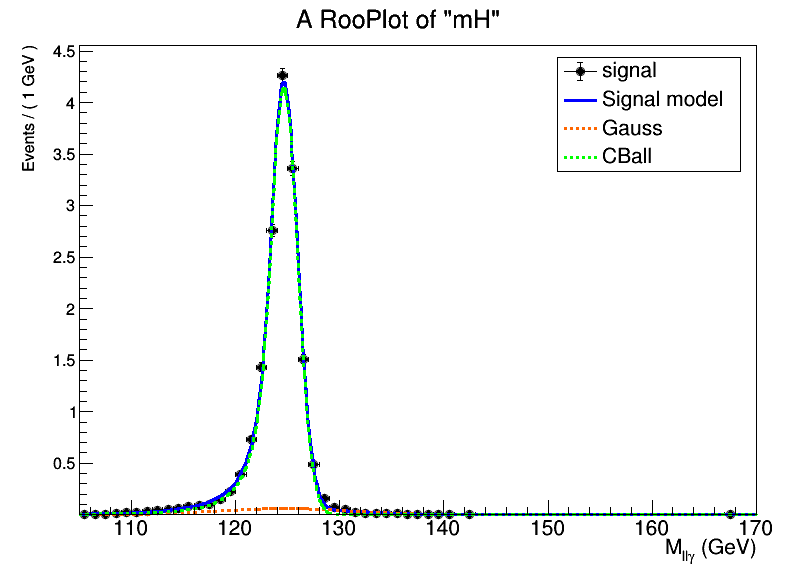
\includegraphics[width=0.40\textwidth]{fig/signal_fit/2018/sigfit_mu_ggF_3_125.png}
		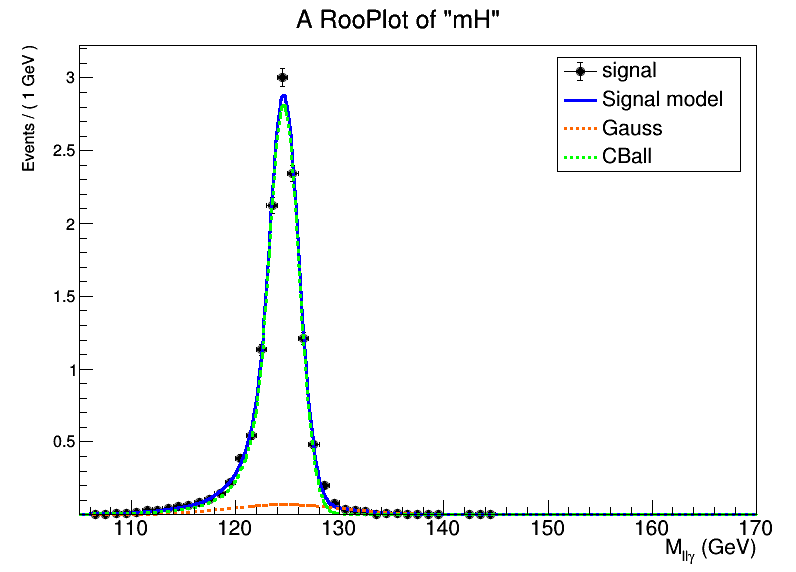
\includegraphics[width=0.40\textwidth]{fig/signal_fit/2018/sigfit_mu_ggF_4_125.png}\\
		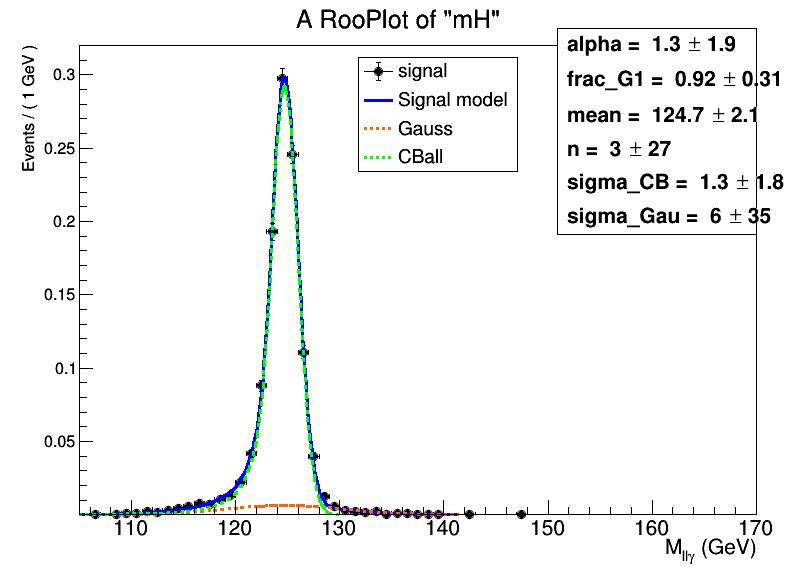
\includegraphics[width=0.40\textwidth]{fig/signal_fit/2018/sigfit_mu_VBF_501_125.png}
		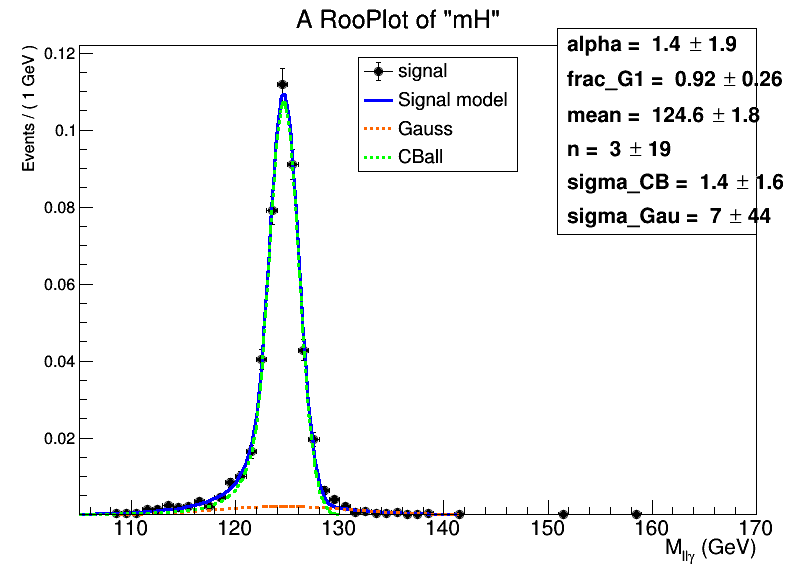
\includegraphics[width=0.40\textwidth]{fig/signal_fit/2018/sigfit_mu_VBF_502_125.png}\\
		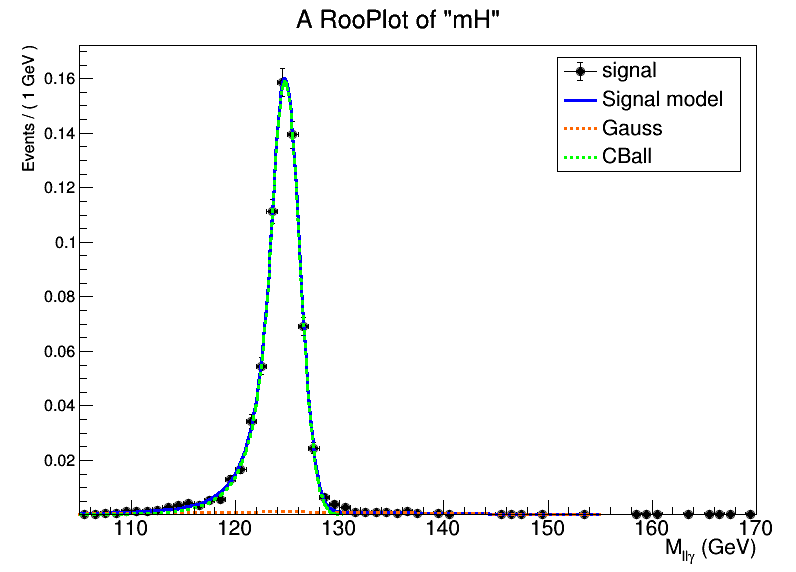
\includegraphics[width=0.40\textwidth]{fig/signal_fit/2018/sigfit_mu_VBF_503_125.png}\\
		\caption{Fits to simulated $m_{\ell^+\ell^-\gamma}$ signal distributions in the muon channel for
            		 $m_\PH=125\GeV$ for the 2018 data-taking period.
			 The top four plots correspond to the untagged categories, and the bottom three plots correspond to the dijet categories.}
		\label{fig:musigfit_18}
	\end{center}
\end{figure}

\begin{figure}[htb]
	\begin{center}
	  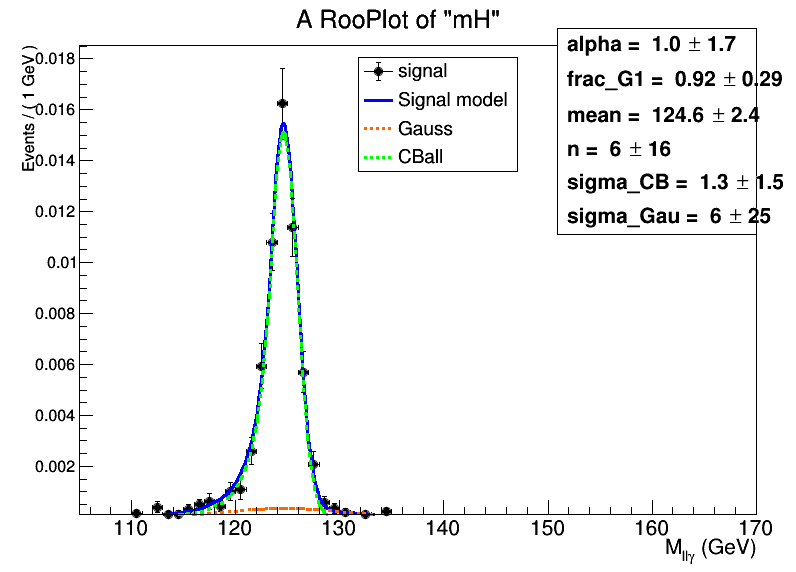
\includegraphics[width=0.30\textwidth]{fig/signal_fit/2016/sigfit_ele_mu_ZH_6789_125.png}
	  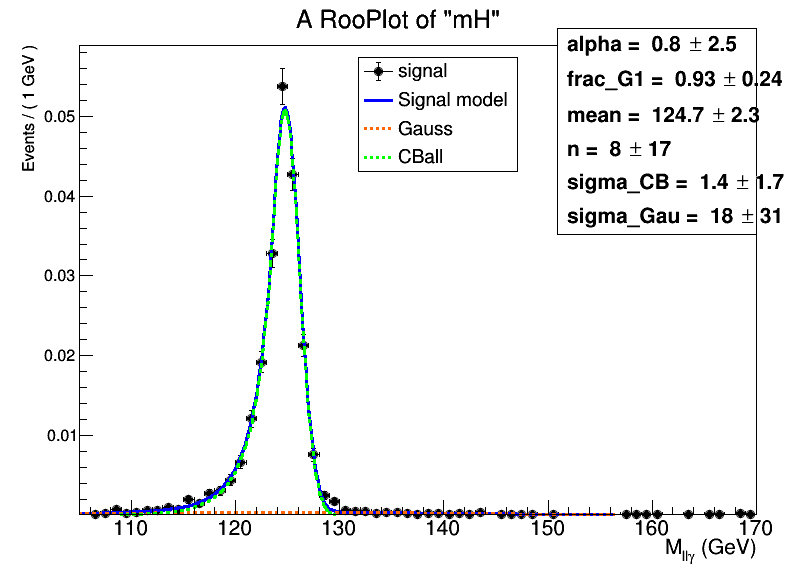
\includegraphics[width=0.30\textwidth]{fig/signal_fit/2016/sigfit_ele_mu_WH_6789_125.png}
		\caption{Fits to simulated $m_{\ell^+\ell^-\gamma}$ signal distributions in the electron and muon channels combined in the lepton-tagged category for
            		 $m_\PH=125\GeV$ for the 2016 data-taking period.
			 The left plot shows the fit to simulated ZH production events, and the right plot shows the fit to simulated WH production events.}
		\label{fig:elemusigfit_16}
	\end{center}
\end{figure}

\begin{figure}[htb]
	\begin{center}
	  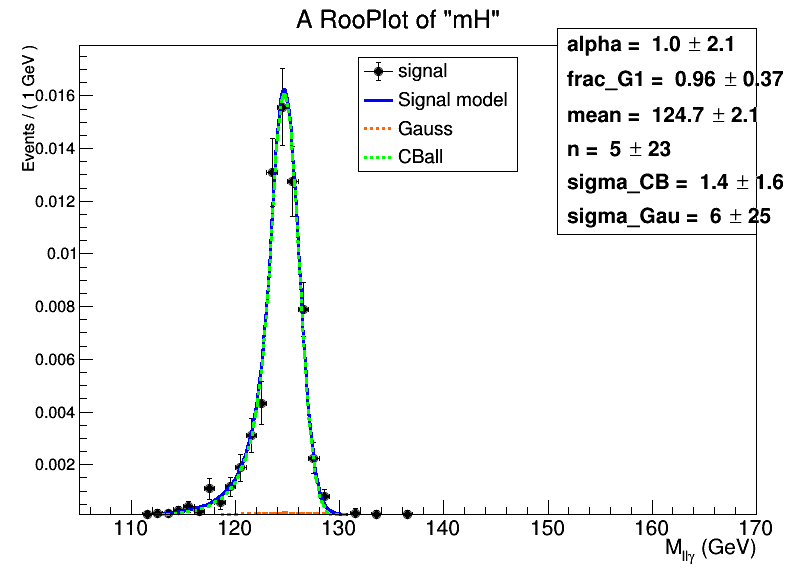
\includegraphics[width=0.30\textwidth]{fig/signal_fit/2017/sigfit_ele_mu_ZH_6789_125.png}
	  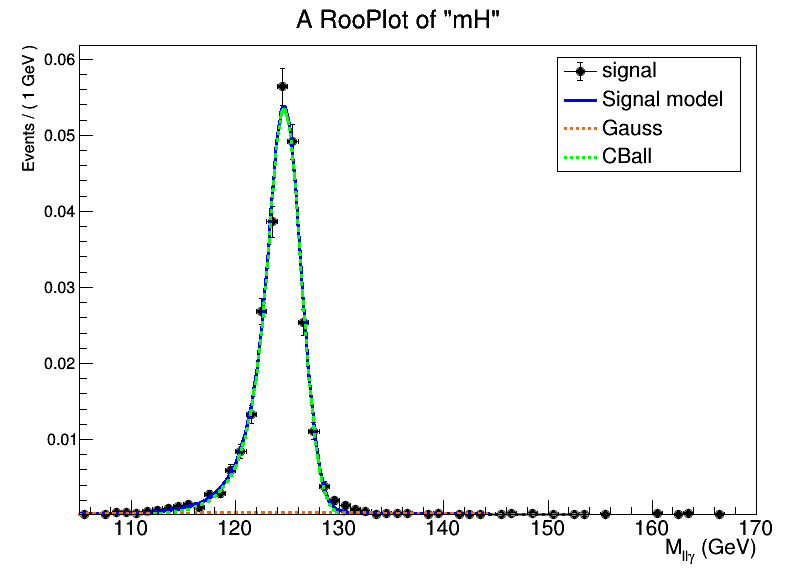
\includegraphics[width=0.30\textwidth]{fig/signal_fit/2017/sigfit_ele_mu_WH_6789_125.png}
		\caption{Fits to simulated $m_{\ell^+\ell^-\gamma}$ signal distributions in the electron and muon channels combined in the lepton-tagged category for
            		 $m_\PH=125\GeV$ for the 2017 data-taking period.
			 The left plot shows the fit to simulated ZH production events, and the right plot shows the fit to simulated WH production events.}
		\label{fig:elemusigfit_17}
	\end{center}
\end{figure}

\begin{figure}[htb]
	\begin{center}
	  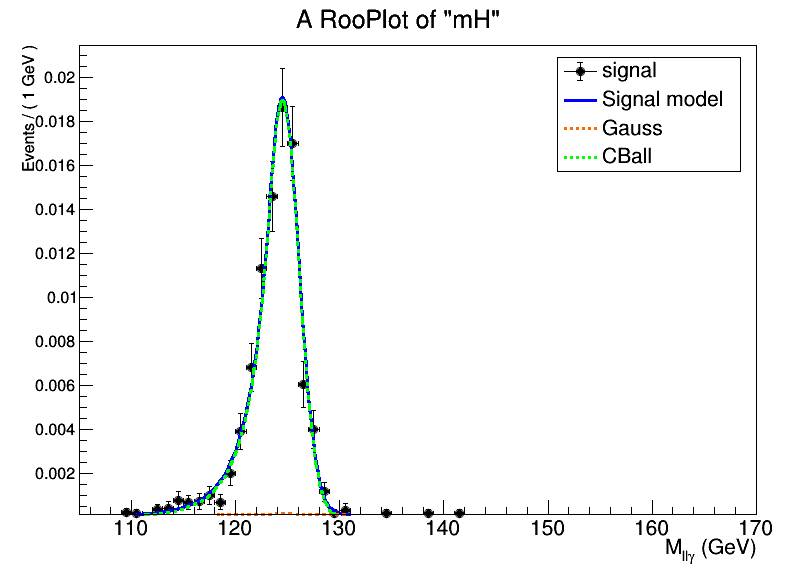
\includegraphics[width=0.30\textwidth]{fig/signal_fit/2018/sigfit_ele_mu_ZH_6789_125.png}
	  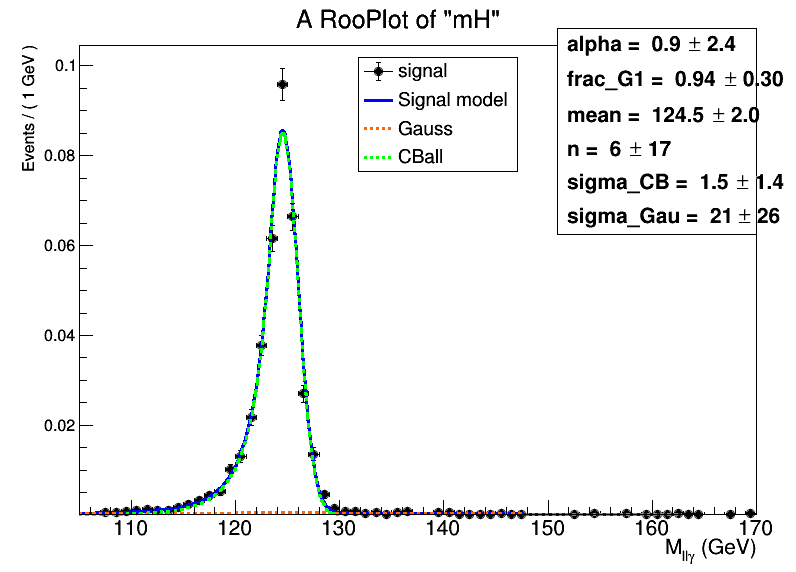
\includegraphics[width=0.30\textwidth]{fig/signal_fit/2018/sigfit_ele_mu_WH_6789_125.png}
		\caption{Fits to simulated $m_{\ell^+\ell^-\gamma}$ signal distributions in the electron and muon channels combined in the lepton-tagged category for
            		 $m_\PH=125\GeV$ for the 2018 data-taking period.
			 The left plot shows the fit to simulated ZH production events, and the right plot shows the fit to simulated WH production events.}
		\label{fig:elemusigfit_18}
	\end{center}
\end{figure}
